\section {Implementation}

\subsection{Prototype}

There are    three  options   for  an in-kernel
implementation of the data plane: (i) OS  native  network stack; (ii) NIC
driver (e.g.,  DPDK~\cite{dpdk});   and  (iii)   customized  in-kernel
software switch (e.g.,  openvswitch~\cite{ovs}).  We chose option (i) because (a) \system has  to choose the  right interface before sending to
the driver   when  having  multiple  interfaces;  and  (b)  a customized
in-kernel software switch has high overhead.  We implement  a kernel module data  plane  and user  space control/management
plane via TCP/UDP sockets, with a total of about 4000 lines of code in
C  and   C++.   We install kernel modules to
register callback  functions with  Linux  \texttt{netfilter}  for data
plane operations. The   control/management  plane  has    extensible,
complex control logic, and the data plane does specific, simpler actions
such as header rewriting, queuing packets to user  space via \texttt{netfilter\_queue} and  updating the
kernel hash table, which holds the flow $\rightarrow$ port mapping.  The user and the kernel  agent  communicate via 
\texttt{netlink}, a native   Linux  Inter Process Communication  (IPC)
function.  Currently the policy server  is   a simple TCP server  that
proactively pushes policies to the agents.

\begin{figure}[ht]
\centering
% 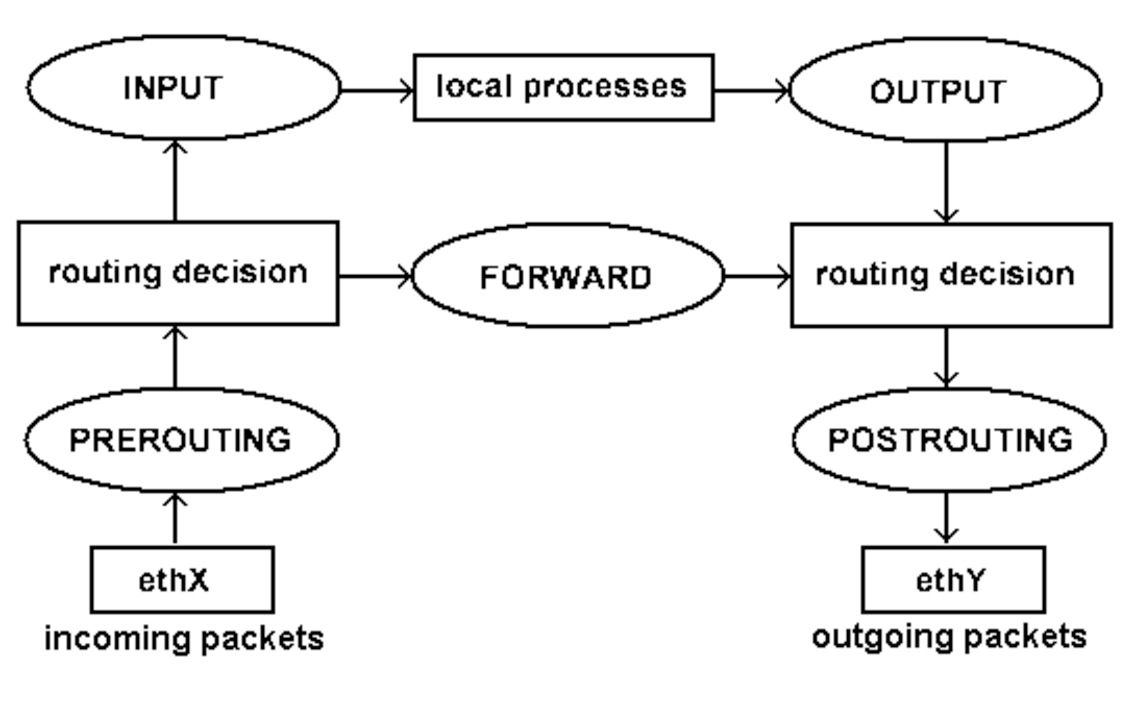
\includegraphics[scale=0.25]{figures/netfilter.pdf} 
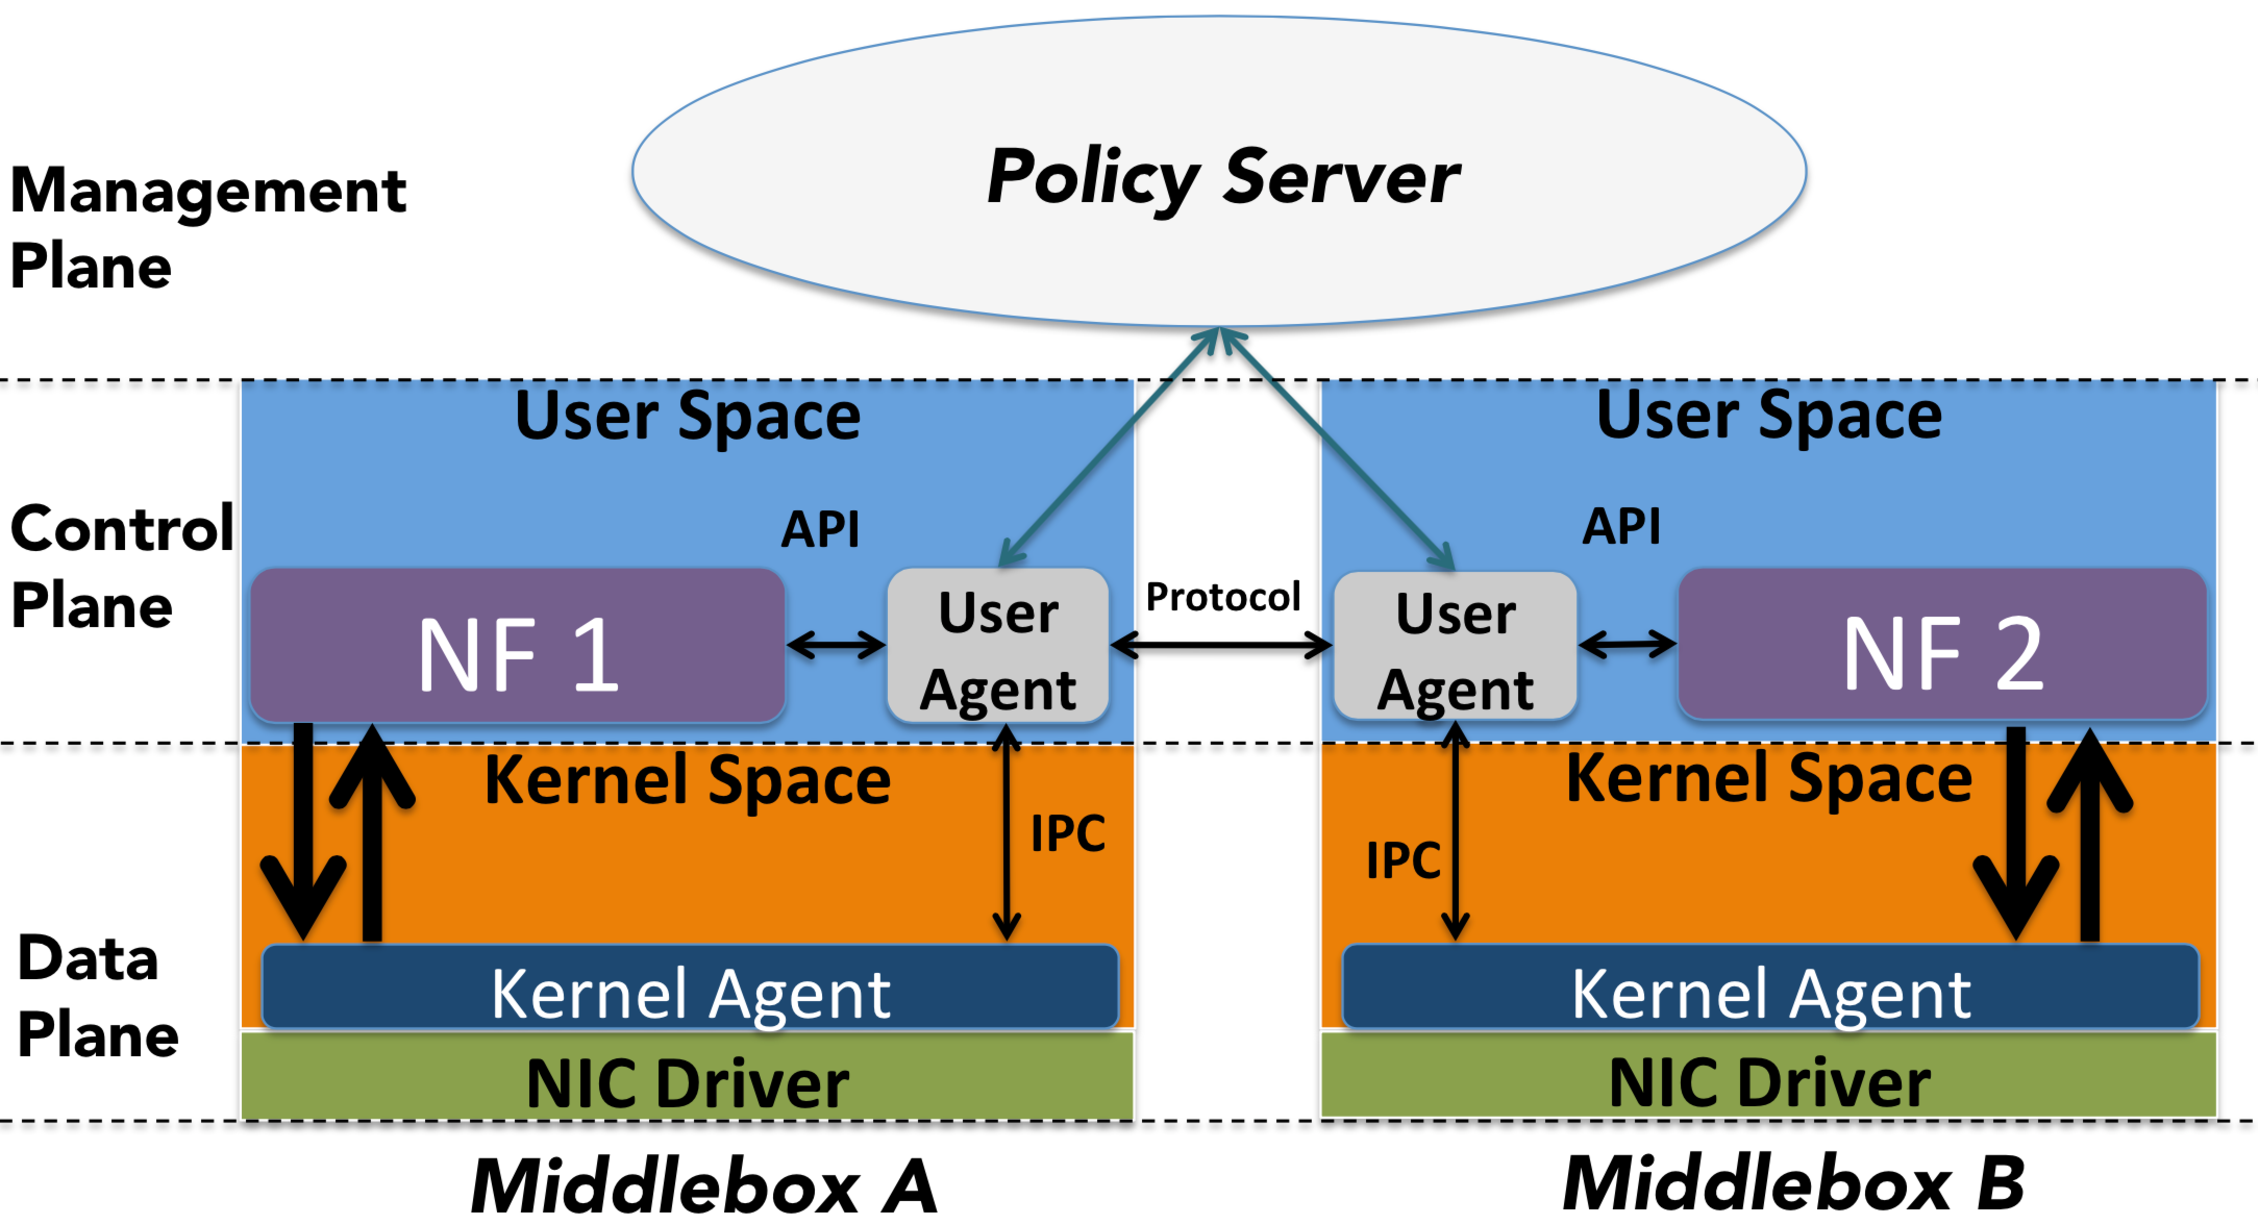
\includegraphics[width=\linewidth]{figures/archiIllustrrate.pdf} 

\caption{\small Layout of the implementation blocks}\label{netf}
\end{figure}





\subsection{Network Function Support}\label{sec:NFsupport}

We categorize NFs into two types --- active and passive functions --- based on whether the NF acts on the original packet.  

\begin{table}[ht]\label{middleboxextension} 
\centering
 
\small
\begin{tabular} {|l |c |c |c|}
\hline

      Name          	  &         Type           & Key        	 &      Binding   \\
                      	  &                        &  Functions          &       Library  \\ \hline
PRADS~\cite{prads} (P) 	  &      Monitoring        &    got\_packet()      & libpcap   \\ \hline
Bro~\cite{bro} (P)      	  &      IDS               &   DumpPacket()      & libpcap   \\ \hline
Snort~\cite{snort} (P)  	  &        IDS         &    PQ\_Show()          & libpcap \\ \hline 
Balance~\cite{balance} (A)	  &      Load Balancer     &    recv(), writen()       &user socket\\ \hline
Squid~\cite{squid} (A) 	  &        Proxy           &  getsockopt()        & user socket  \\ \hline
Traffic- 		  &    WAN-                &     net\_receive       &Linux  \\ 
Squeezer~\cite{tsqueezer} (A)&Optimizer &\_skb()   & skbuff \\ \hline


\end{tabular}
\caption{\small Commonly-used Network Functions; (A) means active and (P) means passive NF. }\label{nfhook}
\end{table}


 Many passive NFs make decisions based on a clone of the original packet. Based on our survey in Table~\ref{nfhook}, we found that most passive NFs use libpcap to capture cloned packets from a raw socket. As described in \S\ref{sec:arch}, we must restore the supersession header of the copies before delivering them to the NF. 
To implement this so-called vertical NAT, we modified the \texttt{pcap\_handle\_packet\_mmap()} function in \texttt{pcap-linux.c} in libpcap~\cite{tcpdump} to restore the supersession. 

For active NFs, there are two cases. If the NFs only act on the payload or MAC layer, e.g.--- TrafficSqueezer, supersession restoring also works. 
However, if the NF acts on the 5-tuple, we have to extend NF functions to notify the \system agent of its header mapping. 
For example, a transparent cache proxy~\cite{squid} gets the packets from its listening port and sets up a new TCP socket to the final destination. \system will break the supersession into two if it is unaware of the mapping between two sessions. On the other hand, if the NF informs the \system agent of the mapping between its listening and sending TCP sockets, the \system agent can stitch the two subsessions into the same supersession. 
 



% \subsection{Middlebox Support}




% 
%Three way handshake
%read write lock
%kmalloc atomic for faster access
